\documentclass[a4paper,12pt]{article}
\usepackage[utf8]{inputenc}
\usepackage[italian]{babel}
\usepackage{graphicx}
\usepackage{amsmath}
\usepackage{caption}
\usepackage{geometry}
\geometry{margin=2.5cm}

\title{La membrana cellulare}
\author{Orcam}
\date{}

\begin{document}

\maketitle

\section*{Funzioni principali delle membrane}

Le membrane biologiche svolgono numerose funzioni fondamentali:
\begin{itemize}
    \item Delimitazione delle cellule e compartimentazione degli organuli.
    \item Mantenimento delle differenze tra l’ambiente intra- ed extracellulare.
    \item Creazione e mantenimento di gradienti ionici e del potenziale di membrana.
    \item Trasferimento di informazioni tramite recettori di superficie.
    \item Supporto a proteine ed enzimi per interazioni con altre cellule e con la matrice extracellulare.
\end{itemize}

\section*{Struttura della membrana plasmatica}

Le membrane biologiche sono costituite da un \textbf{doppio strato fosfolipidico}, arricchito da \textbf{colesterolo} e \textbf{proteine}.

\begin{figure}[h!]
    \centering
    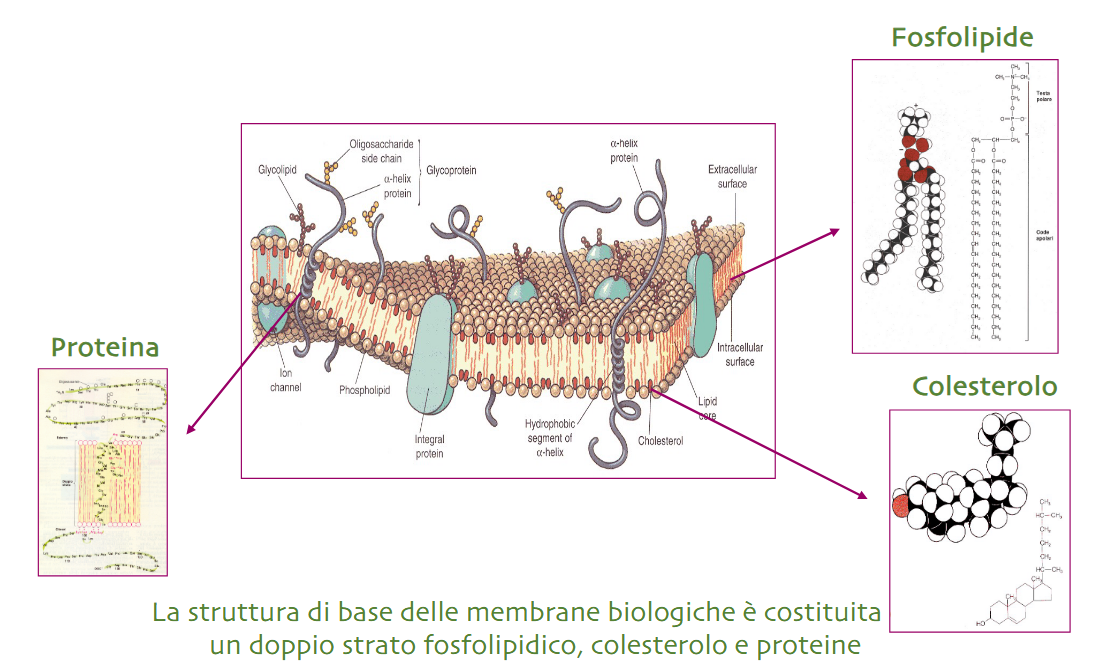
\includegraphics[width=1\textwidth]{Neuroscienze 2024-2025/Modulo I/Screenshot 2025-06-21 at 16-14-45 3. La membrana cellulare.pdf.png}
    \caption{Modello a mosaico fluido di Singer e Nicolson (1972).}
\end{figure}

\subsection*{Componenti lipidiche}
\begin{itemize}
    \item Fosfogliceridi, sfingolipidi, glicolipidi.
    \item Fosfatidilcolina, fosfatidiletanolammina, fosfatidilserina, sfingomielina.
    \item Fosfatidilinositoli: presenti in quantità ridotta ma funzionalmente importanti nella segnalazione intracellulare.
\end{itemize}

\subsection*{Distribuzione asimmetrica}

\begin{itemize}
    \item La distribuzione dei fosfolipidi nei due foglietti della membrana non è simmetrica.
    \item La fosfatidilserina è l’unica carica negativamente a pH fisiologico.
\end{itemize}

\subsection*{Spessore e fluidità}
\begin{itemize}
    \item Spessore medio: 5-10 nm.
    \item Il doppio strato fosfolipidico forma un \textbf{fluido bidimensionale}.
    \item La fluidità dipende da:
    \begin{itemize}
        \item Temperatura.
        \item Lunghezza e insaturazione delle catene aciliche.
        \item Presenza di colesterolo.
    \end{itemize}
\end{itemize}

\section*{Ruolo dei glicolipidi}

\begin{itemize}
    \item Protezione della membrana da condizioni estreme.
    \item Isolamento elettrico (es. nella guaina mielinica).
    \item Coinvolgimento nei processi di riconoscimento cellulare.
\end{itemize}

\section*{Componente proteica}

\subsection*{Tipologie e associazione}
\begin{itemize}
    \item Proteine integrali (passaggio singolo o multiplo).
    \item Proteine periferiche associate tramite:
    \begin{itemize}
        \item Interazioni covalenti (gruppi lipidici).
        \item Interazioni non covalenti con altre proteine o lipidi.
    \end{itemize}
\end{itemize}

\begin{figure}[h!]
    \centering
    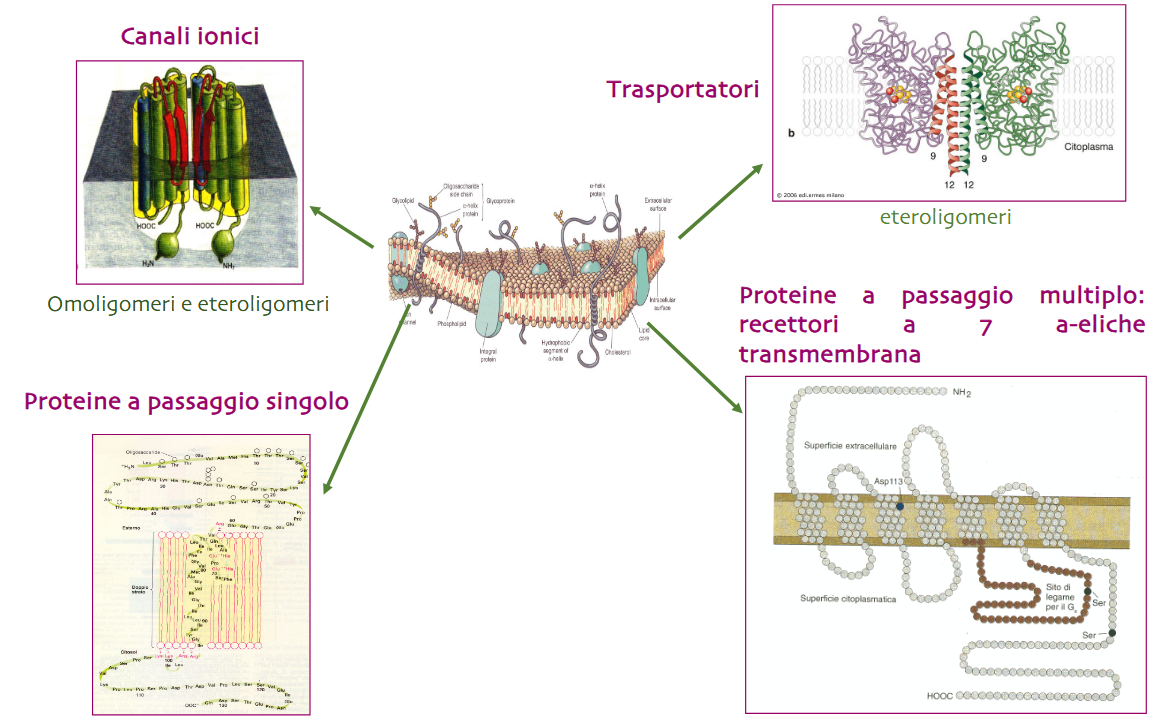
\includegraphics[width=1\textwidth]{Neuroscienze 2024-2025/Modulo I/Screenshot 2025-06-21 at 16-15-19 3. La membrana cellulare.pdf.png}
    \caption{Esempi di proteine transmembrana.}
\end{figure}

\subsection*{Diffusione e organizzazione}

\begin{itemize}
    \item Proteine e lipidi possono essere confinati in \textbf{domini specifici}.
    \item Le proteine della membrana interagiscono con il \textbf{citoscheletro} e la \textbf{matrice extracellulare}.
\end{itemize}

\section*{Il citoscheletro}

\begin{itemize}
    \item Conferisce struttura e forma alla cellula.
    \item Stabilizza la membrana e le sue proteine.
    \item Nei neuroni: impalcatura dei domini cellulari e trasporto di molecole.
\end{itemize}

\subsection*{Tipi di filamenti}
\begin{itemize}
    \item \textbf{Filamenti di actina} (7 nm): funzione dinamica.
    \item \textbf{Filamenti intermedi} (10 nm): funzione statica.
    \item \textbf{Microtubuli} (25 nm): funzione dinamica.
\end{itemize}

\section*{Giunzioni cellulari}

\subsection*{Tipi di legame}
\begin{itemize}
    \item \textbf{Omotipico} (tra cellule simili).
    \item \textbf{Eterotipico} (tra cellule diverse).
\end{itemize}

\subsection*{Tipologie di giunzioni}
\begin{itemize}
    \item \textbf{Giunzioni strette (tight junctions)}: impediscono il passaggio paracellulare e separano domini della membrana.
    \item \textbf{Giunzioni aderenti e desmosomi}: ancorano fortemente le cellule.
    \item \textbf{Gap junctions (giunzioni comunicanti)}: permettono il passaggio diretto di piccoli ioni e molecole tra cellule adiacenti (\textless 500 Dalton).
\end{itemize}

\begin{figure}[h!]
    \centering
    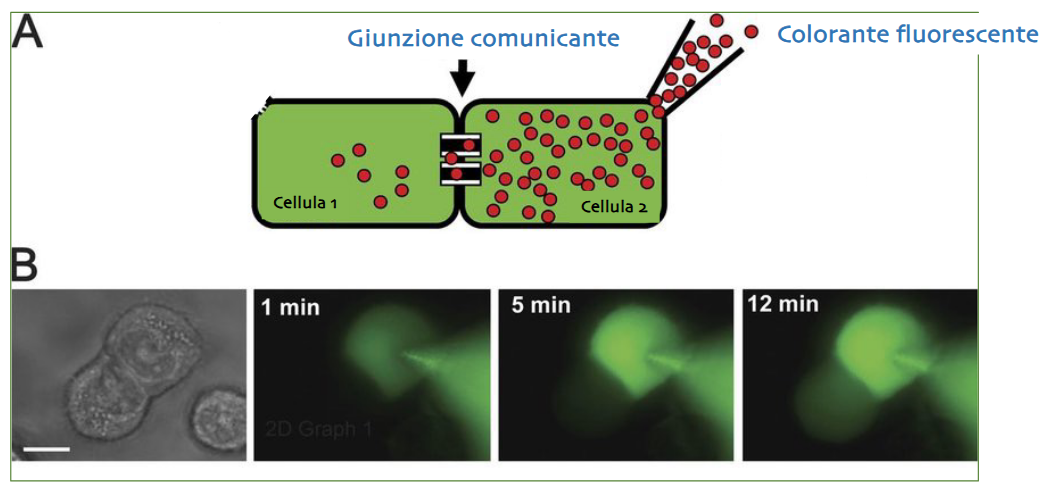
\includegraphics[width=1\textwidth]{Neuroscienze 2024-2025/Modulo I/Screenshot 2025-06-21 at 16-15-48 3. La membrana cellulare.pdf.png}
    \caption{Dimostrazione sperimentale dell’esistenza delle gap junctions.}
\end{figure}

\end{document}
